%%%%%%%%%%%%%%%%%%%%%
% Experiments and Results %
%%%%%%%%%%%%%%%%%%%%%

This thesis aims to analyze the relationships between different road networks and road network similarity methods. In particular,  (1) the similarities between different road networks are determined, (2) similar road networks are clustered, (3) the correlations between the different network similarity methods used to identify the similarities between the different road networks are also determined, and (4) the similar methods are clustered. Figures 4.1 and 4.2 show a high-level overview of the process. 

The problem to find road networks with similar structures and patterns is explicitly approached using network-similarity ranking[Soundarajan]. Firstly, a reference network Gr and a collection of comparison networks H1, H2,...., Hk are given. A network-similarity method is used to calculate the similarity between Gr and each Hi. Second, the comparison networks are clustered and ranked according to how similar they are to the reference network Gr. This step employs the complete-linkage hierarchical clustering method, which generates a dendrogram with many small clusters, providing insight into which road network groups are closely similar or correlated. The clustering results show which groups of road networks have comparable structural and pattern similarities. 

To find methods that behave similarly, Firstly, the pairwise Kendall-Tau distance between each pair of methods is calculated to determine correlations between the different methods which is then followed by a complete-linkage hierarchical clustering because it produces a dendrogram with many small clusters, which provides insight into which groups of methods are closely correlated—the results of this clustering show which groups of methods have similar behavior. 

\begin{figure}[h]
\centering
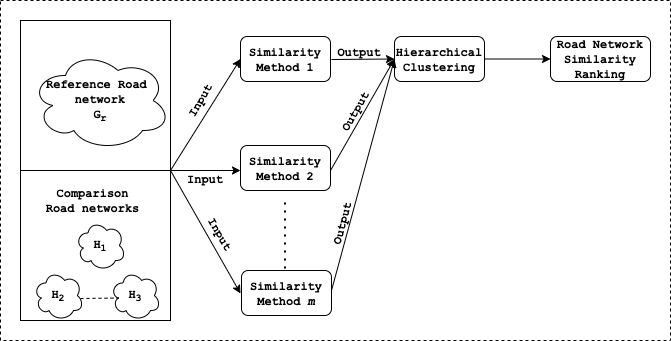
\includegraphics[width=1.25\textwidth,center]{picture/network_ranking.png}
\caption[Miniaturtrichter]{Road Networking Similarity and Ranking}
\label{fig:network ranking}
\end{figure}

\begin{figure}[h]
\centering
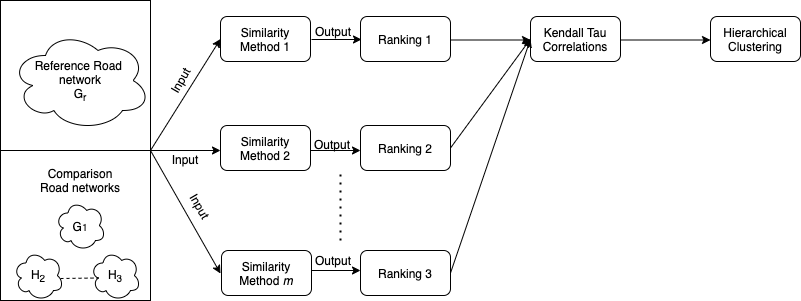
\includegraphics[width=0.55\textwidth,center]{picture/ranking.png}
\caption[Miniaturtrichter]{Road Networking Similarity and Ranking}
\label{fig:network ranking}
\end{figure}


\subsection{Grid Road Network Similarity Analysis}
This section describes the experiments to identify similar road networks with Grid road network patterns and structure, likewise groups of methods described in Section 3 that have similar behavior.
Each method compares two networks and generates a numerical similarity score. This is followed by hierarchical clustering, which generates a dendrogram displaying road network patterns that are similar to the reference road network pattern.

The data (similarity scores) for each comparison are normalized for uniformity before being used to create a dendrogram. This will cancel out the effects of outliers and ensure that the results have the same units. In Table 4.1 that shows the similarity score for each comparison, the normalization is accomplished by calculating Z scores for each similarity score in each column: z = (x mean)/std. As a result, the column mean is subtracted from each value in the column and then divided by the standard deviation. As a result, all the columns have the same mean and variance. The normed values indicate how many standard deviations any individual value deviates from the column mean.
The hierarchical clustering algorithm can now be used in conjunction with the Ward variance minimization algorithm by combining the linkage function to generate the dendrogram.

For the Grid Road Network similarity analysis, the District of Colombia, USA is selected as the reference which other networks as listed in table 4.1 are compared using the similarity methods. Each comparison result is presented in the table.

\begin{figure}[htp]
\centering
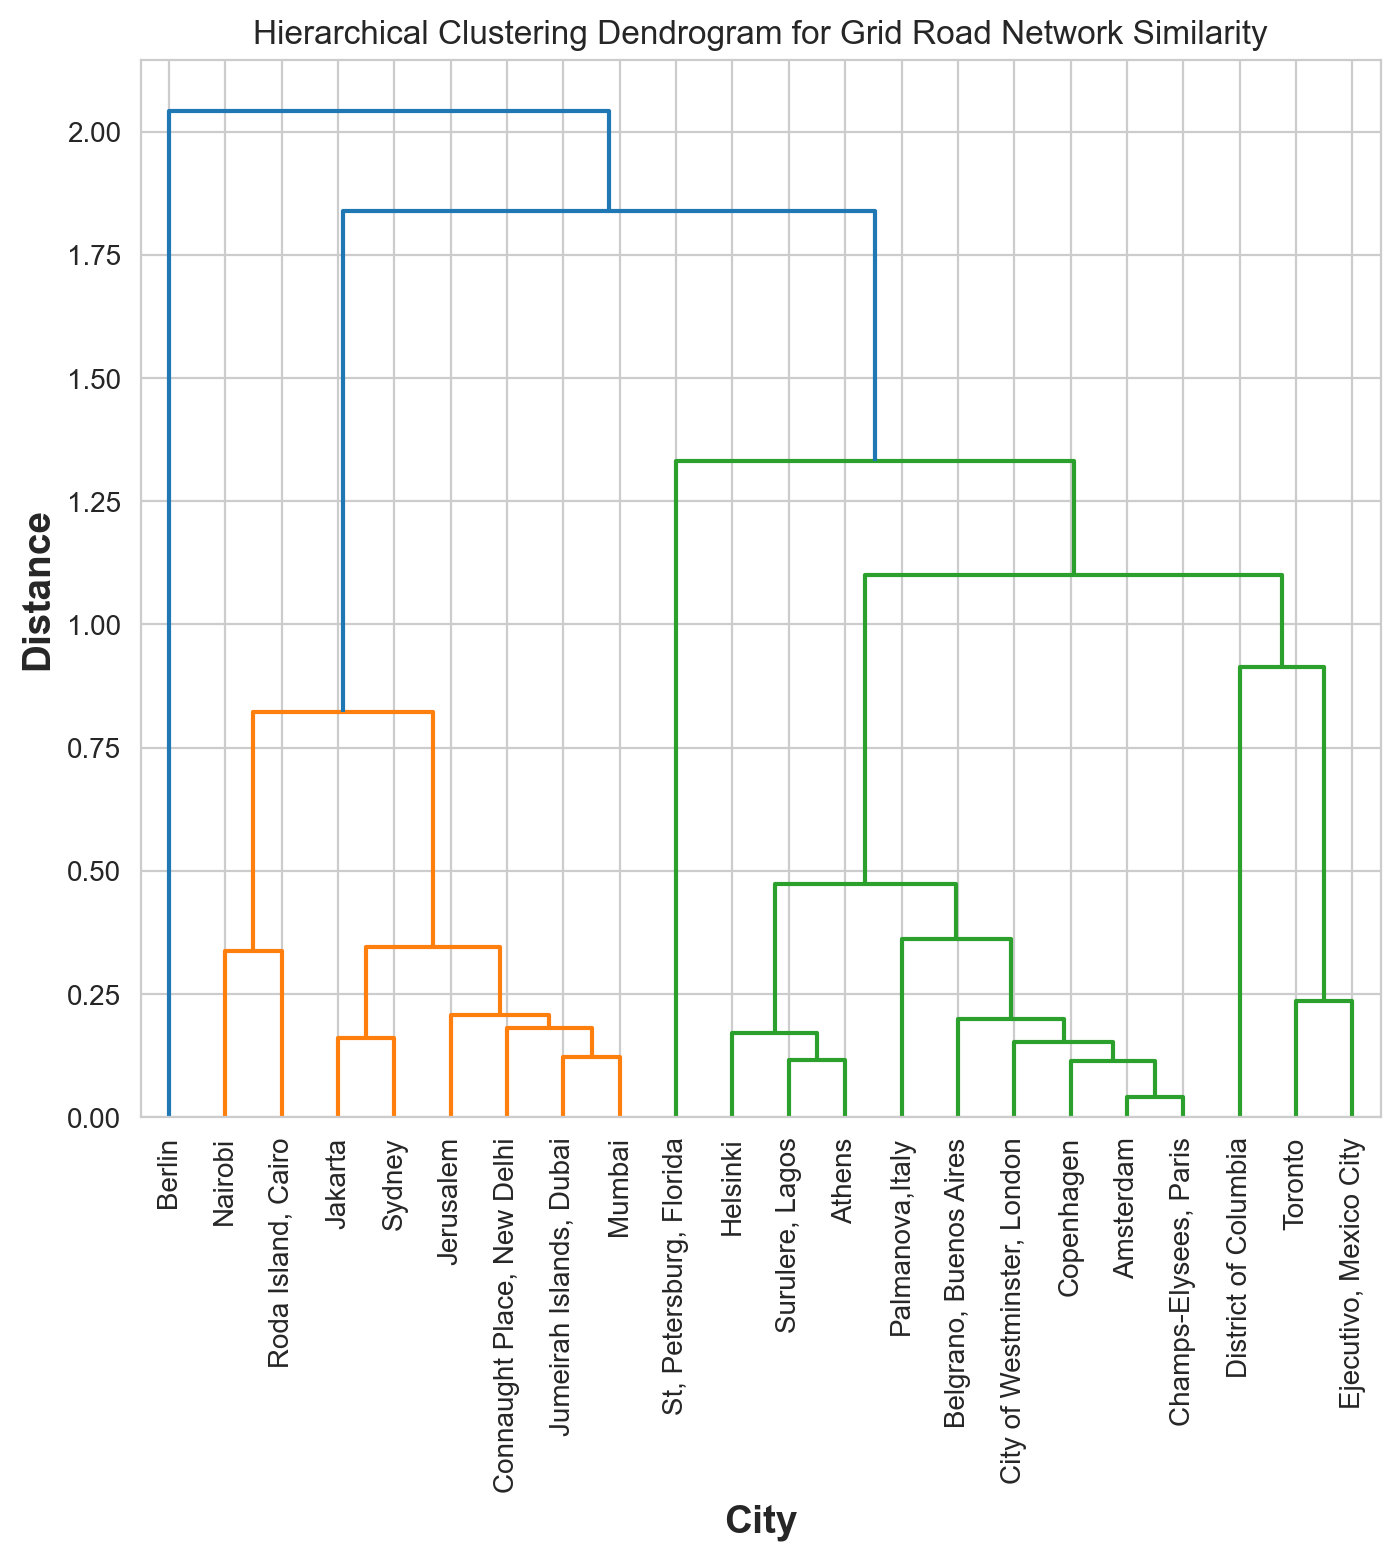
\includegraphics[width=0.75\textwidth,center]{picture/Grid/grid_dendrogram2.png}
\caption[Miniaturtrichter]{Grid Road Networking Similarity}
\label{fig:network ranking}
\end{figure}

The dendrogram created from the analysis shows that there are 4 major clusters in the data identified by running the Ward algorithm on normalized data for all the similarity methods. In general, the overall distances between the clusters are not that large, and with some notable exceptions, the variations within the clusters are relatively small. By cross-checking with the original data table, it is possible to identify the characteristics of the four main groups. 

The first cluster (green in Figure 7) consists of the countries with the similar patterns to the to the reference network largest population, with the Russian Federation as an outlier within the cluster.
The second cluster is made up of wealthy and mostly urbanized countries. Luxembourg stands out as a singleton.
The red cluster contains the majority of the countries: they are neither very rich nor populous. A group of countries with the lowest levels of urbanization can be noted at the bottom of the chart.

Figure 4(a) presents the dendrogram of all of our networks built by hierarchical agglomerative clustering with unweighted
average linking. The network names are labelled on the x-xis. As evident in Figure 4(a), there is a
clear distinction between the clusters. The comparative networks with similar patterns to the reference network appear all together, along with other networks. The Oregon AS forms a cluster that only at the height of 0.45 joins with the Query Log. The Erd os-R enyi and Watts-Strogatz form a separate cluster. This, in turns, reflects our aforementioned intuition about following our background knowledge of the data. Similar results are obtained by applying the x-means clustering on the vectors of local features, for which we report the outcome in Table III. A part from the
distribution of the random networks, the clusters reflect what we observe in Figure 4(a).
Figure 4(b) shows the dendrogram for the above experiment (hierarchical agglomerative clustering with unweighted
average linking and the Canberra Distance) for graph vectors
generated by EIG. This figure clearly shows a different
picture, where the networks are grouped differently (see how
the distribution of the colors is mixed). For example, in the
leftmost cluster, two collaboration networks from arXiv are
put together with four Query Log networks, while the missing
Query Log network is placed together with the Oregon AS
networks. The EIG results are not intuitive, thus making EIG
not suitable for interpreting graph-similarity results.


Firstly, 
We
begin by applying our comparison approaches to the 7
cross-sectional datasets and 20 network similarity methods
described earlier. We consider each of the 7 networks
individually as a reference network. For each reference
network, we produce two baseline networks by
deleting a random 5% of edges and by rewiring a random
5% of edges in such a way as to preserve degree distribution.
We then use the 20 methods to rank the other
8 networks (including the 2 baseline networks) relative
to the reference network. We calculate the Kendall-Tau
distances between each pair of these 20 rankings. The
average Kendall-Tau distance between rankings, over all
networks and all metrics, is 0.28 with a standard deviation
of 0.14. Recall that a distance of 0 indicates perfect
correlation. The average nDCG correlation (with 1 indicating
the highest possible correlation) is 0.93, with
a standard deviation of 0.06. Figure 2 contains the
Kendall-Tau distances between the di↵erent methods
for the case when DBLP was used as a reference graph.
For brevity, we have omitted the heatmap depicting the
nDCG correlations. Surprisingly, the di↵erent methods
are usually correlated with one another even though
they have di↵erent objective functions. Methods RW
and RWR have an average Kendall-Tau distance across
all networks of 0.09, and an average nDCG correlation
of 0.99. This low distance (or alternatively, high correlation)
is expected because the two methods are very similar; but in other cases, the results are more surprising.
For instance, NetSimile and RWR have an average
Kendall-Tau distance of 0.12 and an average nDCG of
0.99, despite having very di↵erent objective functions. 

Next, we cluster the methods using completelinkage
hierarchical clustering on the pairwise Kendall-
Tau distances. Here, we are interested in learning whether groups of complex methods are associated with
simpler, more intuitive methods. For each reference
network, we perform the clustering 1000 times and select
the most common dendrogram. We observe certain
clusters across many of these dendrograms. Table
4 lists clusters observed in four or more clusters out
of the seven considered. Some clusters contain a mix
of both complex as well as simple methods. For example,
RW-Match, RWR-Match, and BFS-Match behave
very much like the much simpler Density method.

This suggests that for frequent network similarity tasks,
one could use the computationally more efficient Density
method as a replacement for these computationally
intensive community-based methods.
Lastly, we apply the Kemeny-Young method to obtain
a single consensus ranking. Table 5 lists the five
similarity methods that are closest to this consensus for
each network, as measured by Kendall-Tau distance.
NetSimile (or one of its variations) and RWR appear
in the top five positions for each network. RWR has
an average Kendall-Tau distance of 0.06 from the consensus,
averaged over all networks. However, RWR has
an average Kendall-Tau distance of 0.21 from the other
similarity methods. This suggests that it is consistently
close to the consensus (i.e., median) ranking, but not
because it is simply close to the other rankings in general.
A user interested in selecting a single representative
method for network similarity ranking should thus
simply select NetSimile or RWR.


\subsection{Radial Road Network Similarity Analysis}
\subsection{Tree Road Network Similarity Analysis}
\subsection{Linear Road Network Similarity Analysis}
\subsection{Cul de Sac Road Network Similarity Analysis}
